% =====================================================================
% Informe IEEE — Hito 2, Etapa 1 · Control Análogo · Universidad del Magdalena
% Compilar con pdfLaTeX (Overleaf: subir este archivo + carpeta figuras/)
% Las marcas [COMPLETAR] indican datos que solo el grupo puede llenar.
% =====================================================================
\documentclass[conference,10pt]{IEEEtran}
\usepackage[utf8]{inputenc}
\usepackage[T1]{fontenc}
\usepackage[spanish,es-noshorthands]{babel}
\usepackage{amsmath,amssymb}
\usepackage{graphicx}
\usepackage{booktabs}
\usepackage{siunitx}
\usepackage{cite}
\usepackage{url}
\sisetup{output-decimal-marker={.}}
\graphicspath{{figuras/}}

\begin{document}

\title{Identificación Dinámica del Monóptero\\ Tower Copter de 1 GDL mediante el\\ Método Fit~3 de Smith y Corripio}

\author{
\IEEEauthorblockN{Nayarit Ramirez, Andru Fonseca}
\IEEEauthorblockA{Programa de Ingeniería Electrónica, Facultad de Ingeniería\\
Universidad del Magdalena, Santa Marta, Colombia\\
Control Análogo — Docente: Ing. Jordan Dallan Guillot Fula, PhD (c)\\
\{[COMPLETAR: correos]\}@unimagdalena.edu.co}
}

\maketitle

\begin{abstract}
Se caracteriza experimentalmente la dinámica vertical de un monóptero (\textit{tower copter}) de un grado de libertad, compuesto por un motor sin escobillas con hélice montado sobre un carro guiado por dos varillas, un controlador electrónico de velocidad (ESC) de \SI{30}{A} y un sensor ultrasónico HC-SR04. Alrededor de un punto de sustentación ($u_0=\SI{1762}{\micro\second}$, $y_0=\SI{13.45}{cm}$) se aplicó un escalón de \SI{50}{\micro\second} en el ancho de pulso, con muestreo determinístico de \SI{50}{ms}. Aplicando el método de dos puntos Fit~3 de Smith y Corripio sobre la curva de reacción filtrada se obtuvo el modelo de primer orden con tiempo muerto $G_p(s)=0.4302\,e^{-0.1188s}/(1.5719s+1)$ [cm/\si{\micro\second}], con un porcentaje de ajuste de \SI{85.77}{\percent} y un RMSE de \SI{0.754}{cm}, superior al criterio de aceptación (\SI{80}{\percent}). Se analizan los residuos, las fuentes de error (ruido y ecos espurios del ultrasonido, deriva del punto de operación) y las implicaciones del modelo para el diseño del controlador PID de la Etapa~2.
\end{abstract}

\begin{IEEEkeywords}
Identificación de sistemas, FOPDT, método Fit~3, monóptero, tower copter, linealización, HC-SR04.
\end{IEEEkeywords}

% ---------------------------------------------------------------------
\section{Introducción}
El monóptero de un grado de libertad es una planta didáctica clásica para el estudio del control continuo: un actuador aerodinámico (motor y hélice) sostiene un carro que se desplaza verticalmente a lo largo de guías. Su dinámica es no lineal, pues el empuje crece con el cuadrado de la velocidad angular de la hélice, y presenta zonas de comportamiento muy distinto: una zona muerta en la que el carro permanece apoyado sobre los resortes de la base y una zona superior en la que la cercanía del travesaño altera el flujo de aire.

Para aplicar la teoría de control lineal es necesario obtener un modelo válido alrededor de un punto de operación. Este trabajo, correspondiente a la Etapa~1 del proyecto, tiene como objetivo identificar un modelo de primer orden con tiempo muerto (FOPDT) alrededor del punto de sustentación (\textit{hovering}) mediante el método de dos puntos Fit~3 de Smith y Corripio~\cite{smith}, y validarlo frente a la respuesta experimental mediante el porcentaje de ajuste (Fit) y el error cuadrático medio (RMSE), según la guía del curso~\cite{guia}.

% ---------------------------------------------------------------------
\section{Fundamentos teóricos}

\subsection{Dinámica del sistema}
Aplicando la segunda ley de Newton al carro de masa $m$~\cite{ogata}:
\begin{equation}
m\,\ddot y + B\,\dot y + m g = F_t(u), \qquad F_t \propto \omega^2 \propto u^2 ,
\label{eq:newton}
\end{equation}
donde $y$ es la altura, $B$ el coeficiente de fricción viscosa de las guías y del aire, y $u$ el ancho de pulso enviado al ESC. Mientras $F_t < mg$ el carro permanece en reposo sobre la base (zona muerta).

\subsection{Linealización en el punto de sustentación}
En el punto de operación $(u_0, y_0)$ el empuje equilibra el peso, $F_t(u_0)=mg$. Definiendo las variables incrementales $\Delta u=u-u_0$ y $\Delta y = y-y_0$, y desarrollando $F_t$ en serie de Taylor de primer orden, se obtiene un modelo lineal válido para perturbaciones pequeñas. Trabajar por encima de la base evita además el efecto suelo, que distorsiona el empuje cuando la hélice está muy cerca de una superficie.

\subsection{Modelo de primer orden con tiempo muerto}
Aunque \eqref{eq:newton} es de segundo orden, la fricción viscosa de las guías y la respuesta aerodinámica hacen que un polo domine sobre el otro, por lo que la planta puede aproximarse por
\begin{equation}
G_p(s)=\frac{\Delta Y(s)}{\Delta U(s)} = \frac{K\,e^{-t_0 s}}{\tau s + 1},
\label{eq:fopdt}
\end{equation}
donde $K$ es la ganancia estática, $\tau$ la constante de tiempo y $t_0$ el tiempo muerto aparente, que agrupa la respuesta del ESC, la aceleración angular de la hélice y la latencia de medición. Su respuesta ante un escalón de amplitud $\Delta u$ es
\begin{equation}
\Delta y(t) = K\,\Delta u \left[1-e^{-(t-t_0)/\tau}\right]\,\mathbf{1}(t-t_0).
\label{eq:respuesta}
\end{equation}

\subsection{Método Fit~3 de Smith y Corripio}
Normalizando \eqref{eq:respuesta} por su valor final, $F(t)=1-e^{-(t-t_0)/\tau}$. Los instantes en que la respuesta alcanza el \SI{28.3}{\percent} y el \SI{63.2}{\percent} cumplen
\begin{align}
0.283 &= 1-e^{-(t_1-t_0)/\tau} \;\Rightarrow\; t_1-t_0 = \tau\ln\tfrac{1}{0.717} \approx \tfrac{\tau}{3},\\
0.632 &= 1-e^{-(t_2-t_0)/\tau} \;\Rightarrow\; t_2-t_0 = \tau .
\end{align}
Restando ambas expresiones se obtienen las fórmulas del método:
\begin{equation}
\tau = \tfrac{3}{2}(t_2-t_1), \qquad t_0 = t_2-\tau, \qquad K=\frac{\Delta y}{\Delta u}.
\label{eq:fit3}
\end{equation}

% ---------------------------------------------------------------------
\section{Metodología experimental}

\subsection{Banco experimental}
El banco (Fig.~\ref{fig:banco}) consta de un marco de madera con dos varillas de acero que guían un carro de madera; sobre él va el motor sin escobillas con su hélice. El ESC de \SI{30}{A} se alimenta con una fuente regulada de \SI{12}{V}/\SI{5}{A}. La altura se mide con un sensor ultrasónico HC-SR04 ubicado en la base y apuntando hacia el carro. Un Arduino Uno genera el PWM del ESC en el pin~D9 (\num{1000}--\SI{2000}{\micro\second}), dispara el sensor por D7/D6 y transmite los datos por USB a \SI{115200}{baudios}, con masa común entre todos los equipos (Fig.~\ref{fig:conexiones}). El recorrido útil es de \SI{100}{cm}: el carro descansa sobre los resortes a $\approx$\SI{11}{cm} de lectura del sensor.

\begin{figure}[t]
\centering
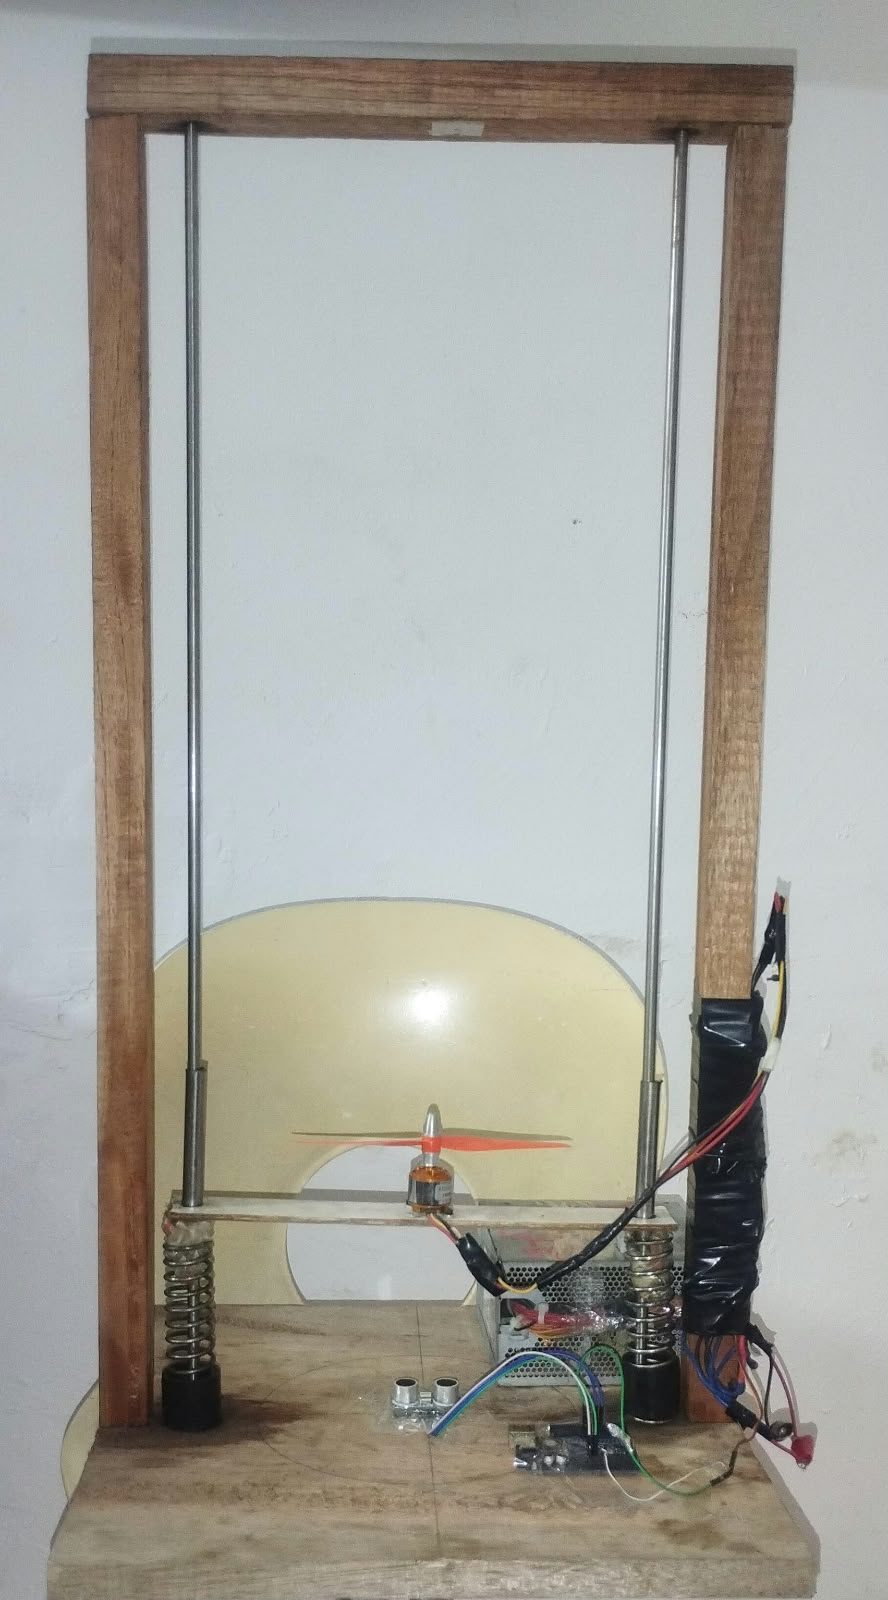
\includegraphics[height=6.4cm]{monocoptero-real.jpg}\hfill
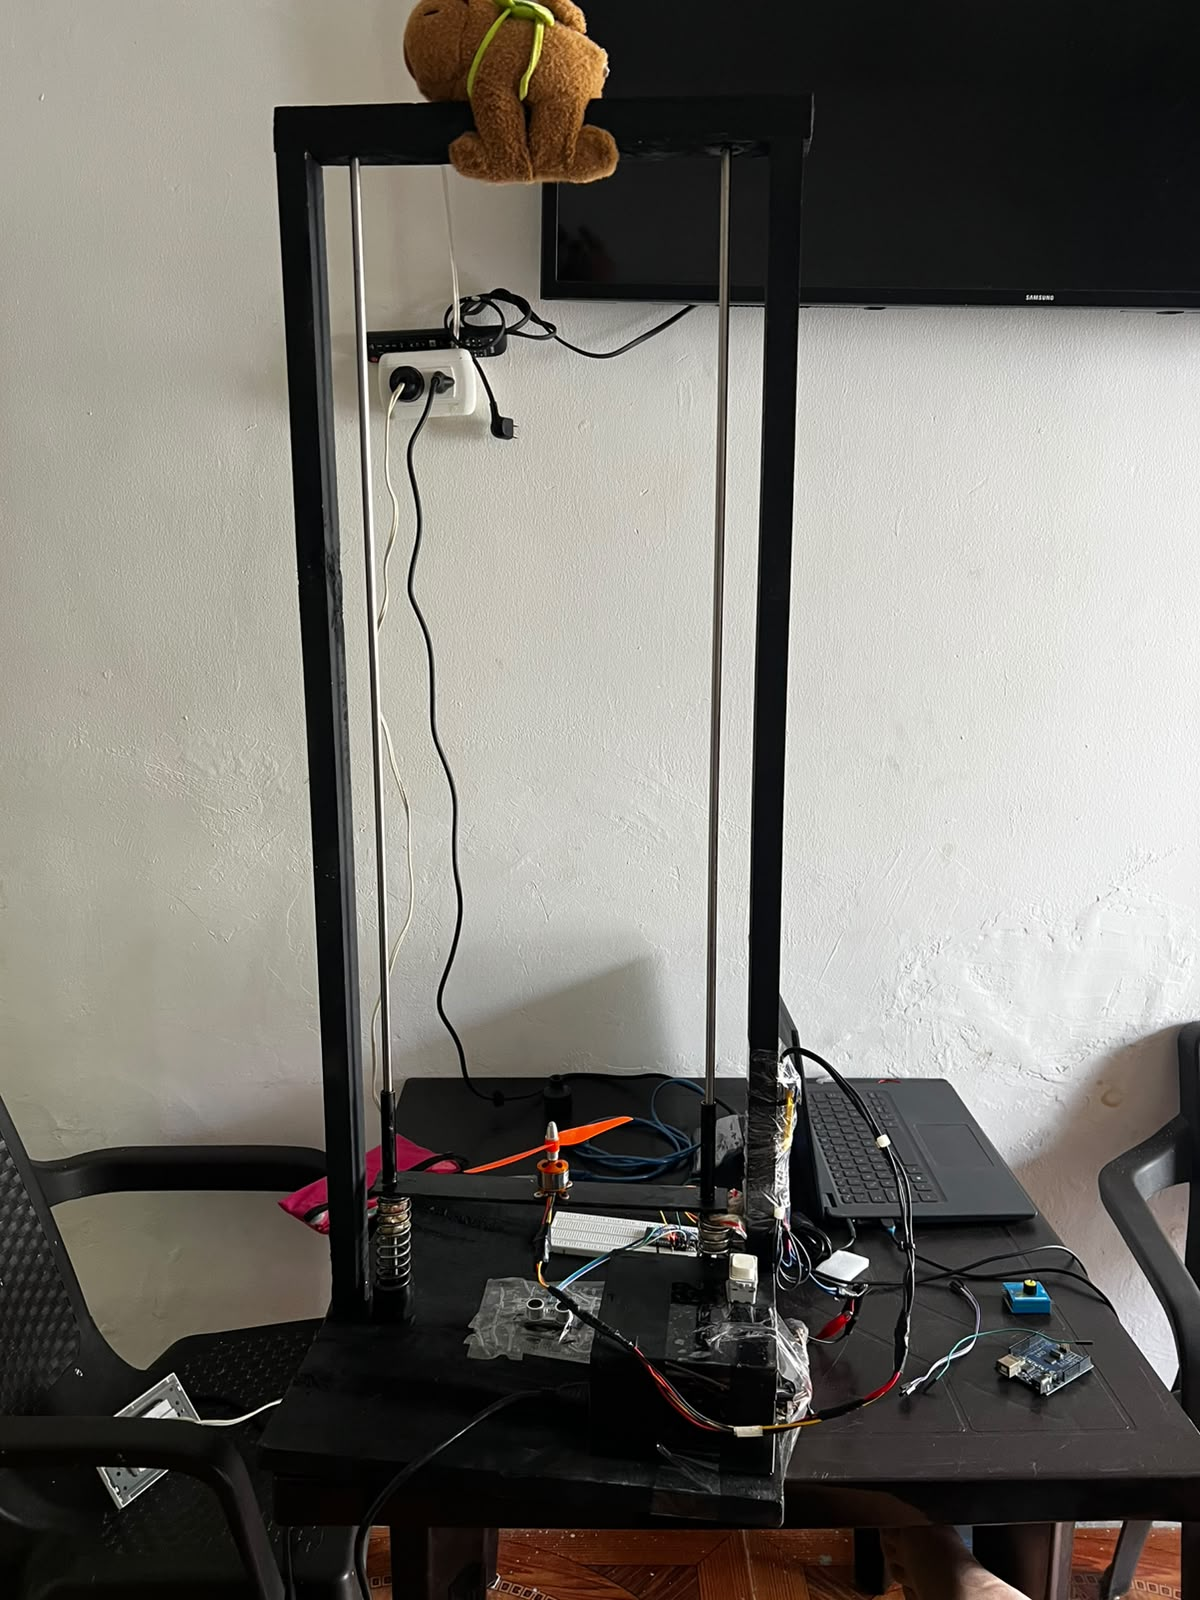
\includegraphics[height=6.4cm]{banco_actual.jpg}
\caption{Banco experimental del monóptero de 1 GDL. Izquierda: montaje original. Derecha: estado actual del banco (1 de octubre de 2026).}
\label{fig:banco}
\end{figure}

\begin{figure}[t]
\centering
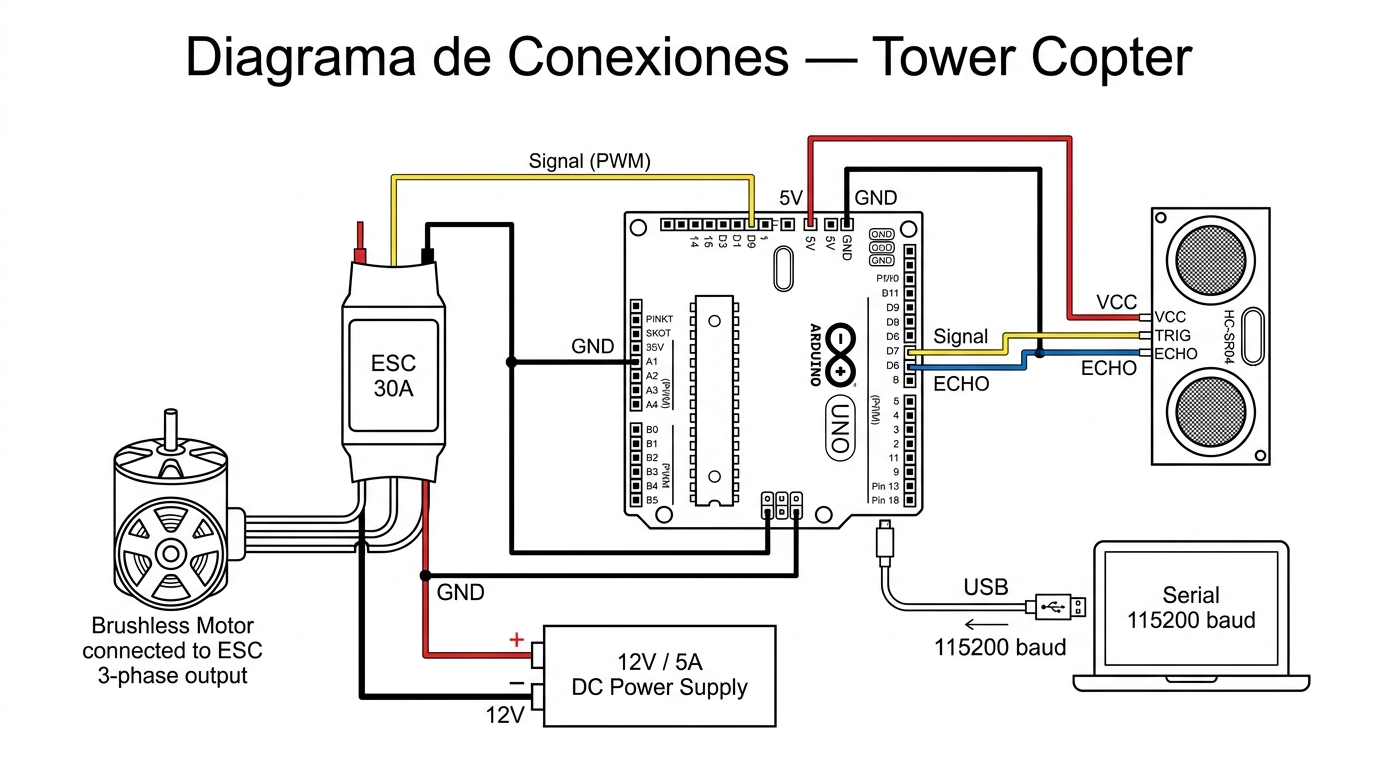
\includegraphics[width=\columnwidth]{diagrama_conexiones.jpg}
\caption{Diagrama de conexiones del banco.}
\label{fig:conexiones}
\end{figure}

\subsection{Protocolo de armado del ESC y seguridad}
Al encender se envía la secuencia de calibración \SI{1000}{\micro\second} (\SI{2}{s}) $\rightarrow$ \SI{2000}{\micro\second} (\SI{2}{s}) $\rightarrow$ \SI{1000}{\micro\second} (\SI{2}{s}) con la hélice despejada. El firmware incluye un \textit{failsafe} que lleva el PWM a \SI{1000}{\micro\second} si la altura supera \SI{85}{cm}, y el ensayo se realiza con el operador fuera del alcance de la hélice.

\subsection{Estrategia de captura}
El firmware usa un periodo de muestreo determinístico $T_s=\SI{50}{ms}$ basado en \texttt{millis()}. El ensayo dura \SI{15}{s}: durante los primeros \SI{5}{s} mantiene $u_0=\SI{1762}{\micro\second}$ para estabilizar el carro en sustentación; luego aplica el escalón a \SI{1812}{\micro\second} ($\Delta u=+\SI{50}{\micro\second}$) durante \SI{10}{s} y finalmente apaga el motor. Cada muestra se envía como \texttt{tiempo\_ms,pwm\_us,altura\_cm}; se registraron 299 muestras sin pérdidas (archivo \texttt{datos\_escalon\_20260913\_193329.csv}).

\subsection{Procesamiento}
El script \texttt{IdentificacionFIT3.m}: (i) aplica un filtro de mediana de orden~5 (\texttt{medfilt1}), que elimina los valores atípicos del ultrasonido sin desplazar la fase, por lo que no altera $t_0$; (ii) detecta el escalón en $u(t)$ y redefine el tiempo como relativo a ese instante ($t=0$), evitando el error de usar el tiempo absoluto de \texttt{millis()}; (iii) estima $u_0,y_0$ con el promedio previo al escalón y $u_\infty,y_\infty$ con el último \SI{15}{\percent} del registro; (iv) interpola linealmente el primer cruce de los niveles \SI{28.3}{\percent} y \SI{63.2}{\percent} y aplica \eqref{eq:fit3}; (v) simula \eqref{eq:respuesta}, verifica el resultado con \texttt{lsim} y calcula las métricas
\begin{equation}
\mathrm{Fit}=\left(1-\frac{\lVert y-\hat y\rVert}{\lVert y-\bar y\rVert}\right)\!\times 100\%,\quad
\mathrm{RMSE}=\sqrt{\tfrac{1}{N}\textstyle\sum (y-\hat y)^2}.
\end{equation}

% ---------------------------------------------------------------------
\section{Resultados y análisis}

\subsection{Punto de operación y curva de reacción}
La Fig.~\ref{fig:fit3} muestra el ensayo completo. Antes del escalón el carro se sostiene alrededor de $y_0=\SI{13.45}{cm}$; tras el escalón sube de forma aperiódica, sin oscilaciones ni sobreimpulso, hasta $y_\infty=\SI{34.96}{cm}$, el comportamiento esperado de un sistema de primer orden.

\begin{figure}[t]
\centering
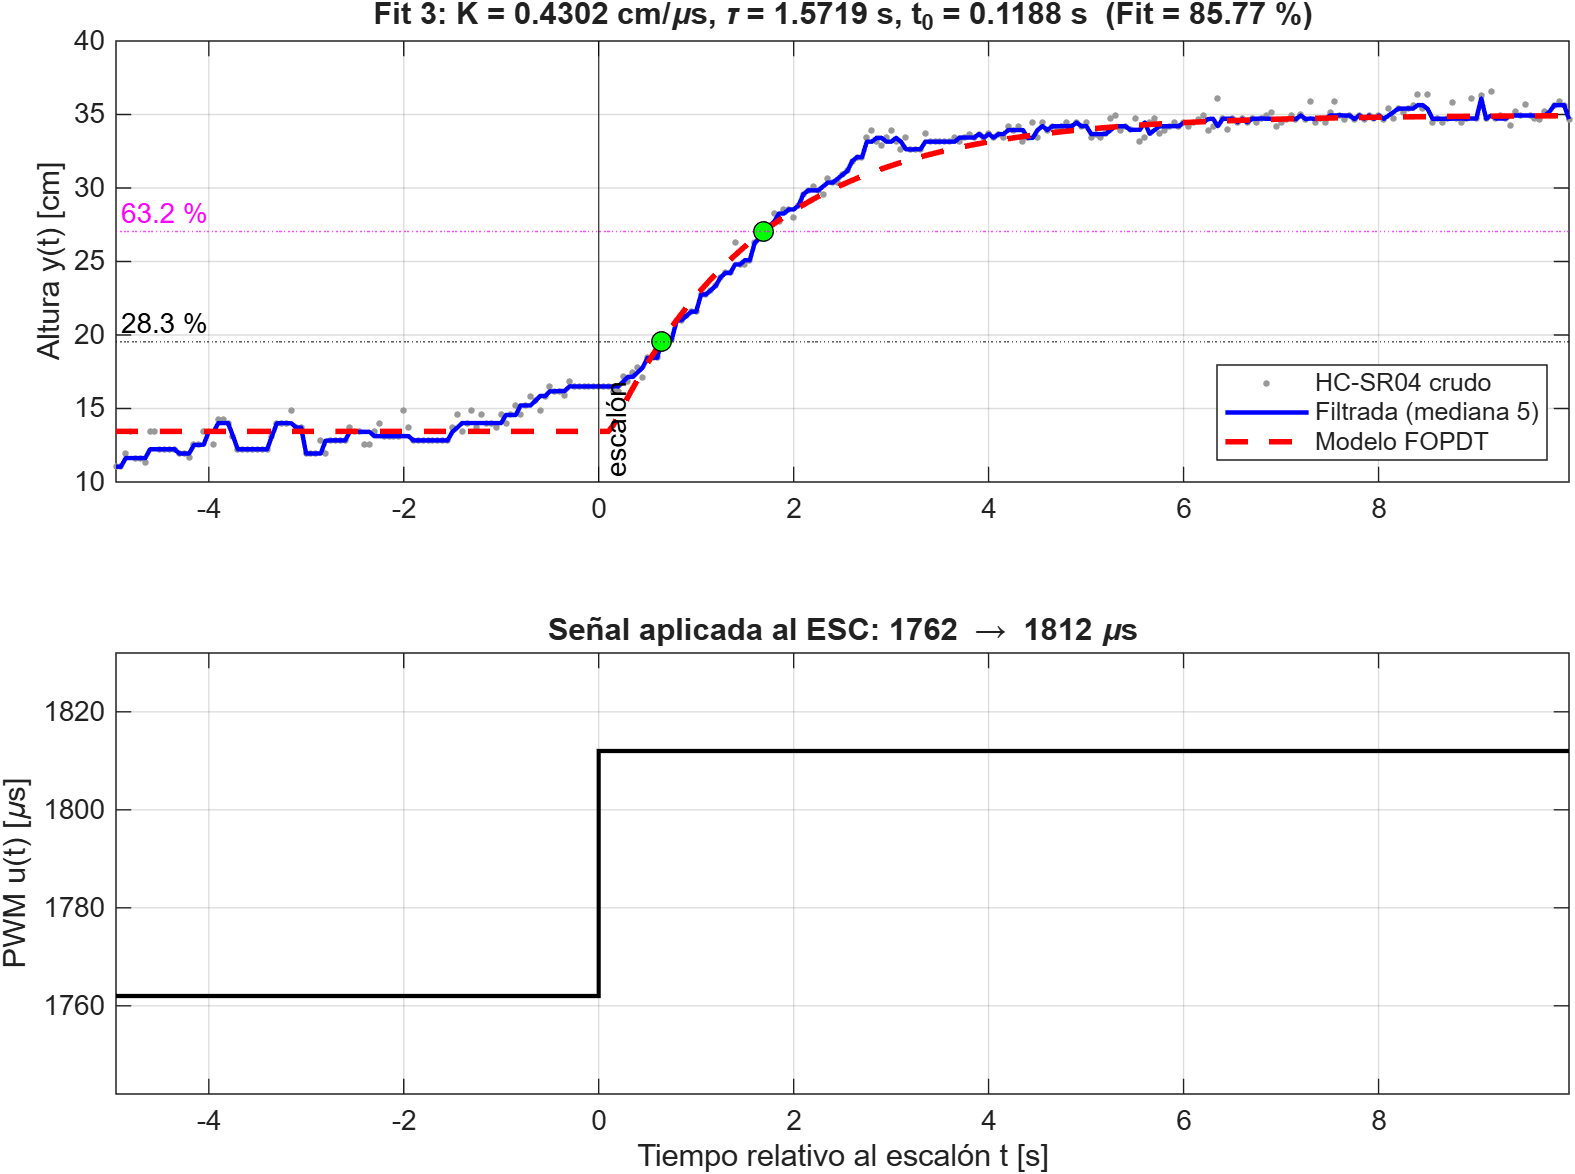
\includegraphics[width=\columnwidth]{fit3_respuesta.png}
\caption{Ensayo completo (t = 0 en el escalón): lectura cruda del HC-SR04, señal filtrada, modelo FOPDT y puntos del 28.3\,\% y 63.2\,\% (arriba); PWM aplicado al ESC (abajo).}
\label{fig:fit3}
\end{figure}

\subsection{Cálculo de los parámetros}
Con $\Delta u=\SI{50}{\micro\second}$ y $\Delta y=\SI{21.51}{cm}$, los niveles de referencia son $y_{28.3}=\SI{19.53}{cm}$ y $y_{63.2}=\SI{27.04}{cm}$, alcanzados en $t_1=\SI{0.6427}{s}$ y $t_2=\SI{1.6906}{s}$. Aplicando \eqref{eq:fit3}:
\begin{align*}
K &= 21.51/50 = \SI{0.4302}{cm/\micro\second},\\
\tau &= 1.5\,(1.6906-0.6427) = \SI{1.5719}{s},\\
t_0 &= 1.6906-1.5719 = \SI{0.1188}{s}.
\end{align*}
El modelo identificado es
\begin{equation}
G_p(s)=\frac{0.4302\,e^{-0.1188 s}}{1.5719 s+1}\quad\left[\frac{\text{cm}}{\si{\micro\second}}\right],
\end{equation}
con un polo en $s=-1/\tau=\SI{-0.6362}{rad/s}$ en el semiplano izquierdo (Fig.~\ref{fig:polos}): la planta es estable en lazo abierto, con un tiempo de establecimiento (\SI{2}{\percent}) de \SI{6.27}{s}. La Tabla~\ref{tab:res} resume los resultados.

\begin{table}[t]
\centering
\caption{Resultados de la identificación}
\label{tab:res}
\begin{tabular}{@{}llr@{}}
\toprule
Símbolo & Descripción & Valor \\ \midrule
$u_0$ & PWM de sustentación & \SI{1762.00}{\micro\second} \\
$y_0$ & Altura de sustentación & \SI{13.45}{cm} \\
$u_\infty$ & PWM final & \SI{1812.00}{\micro\second} \\
$y_\infty$ & Altura final & \SI{34.96}{cm} \\
$t_1$, $t_2$ & Instantes del 28.3\,\% y 63.2\,\% & \SI{0.6427}{s}, \SI{1.6906}{s} \\
$K$ & Ganancia estática & \SI{0.4302}{cm/\micro\second} \\
$\tau$ & Constante de tiempo & \SI{1.5719}{s} \\
$t_0$ & Tiempo muerto & \SI{0.1188}{s} \\
$p$ & Polo dominante & \SI{-0.6362}{rad/s} \\
RMSE & Error cuadrático medio & \SI{0.7540}{cm} \\
$|e|_{\max}$ & Error máximo & \SI{3.05}{cm} \\
Fit & Ajuste (señal filtrada) & \SI{85.77}{\percent} \\
Fit & Ajuste (señal cruda) & \SI{84.02}{\percent} \\ \bottomrule
\end{tabular}
\end{table}

\begin{figure}[t]
\centering
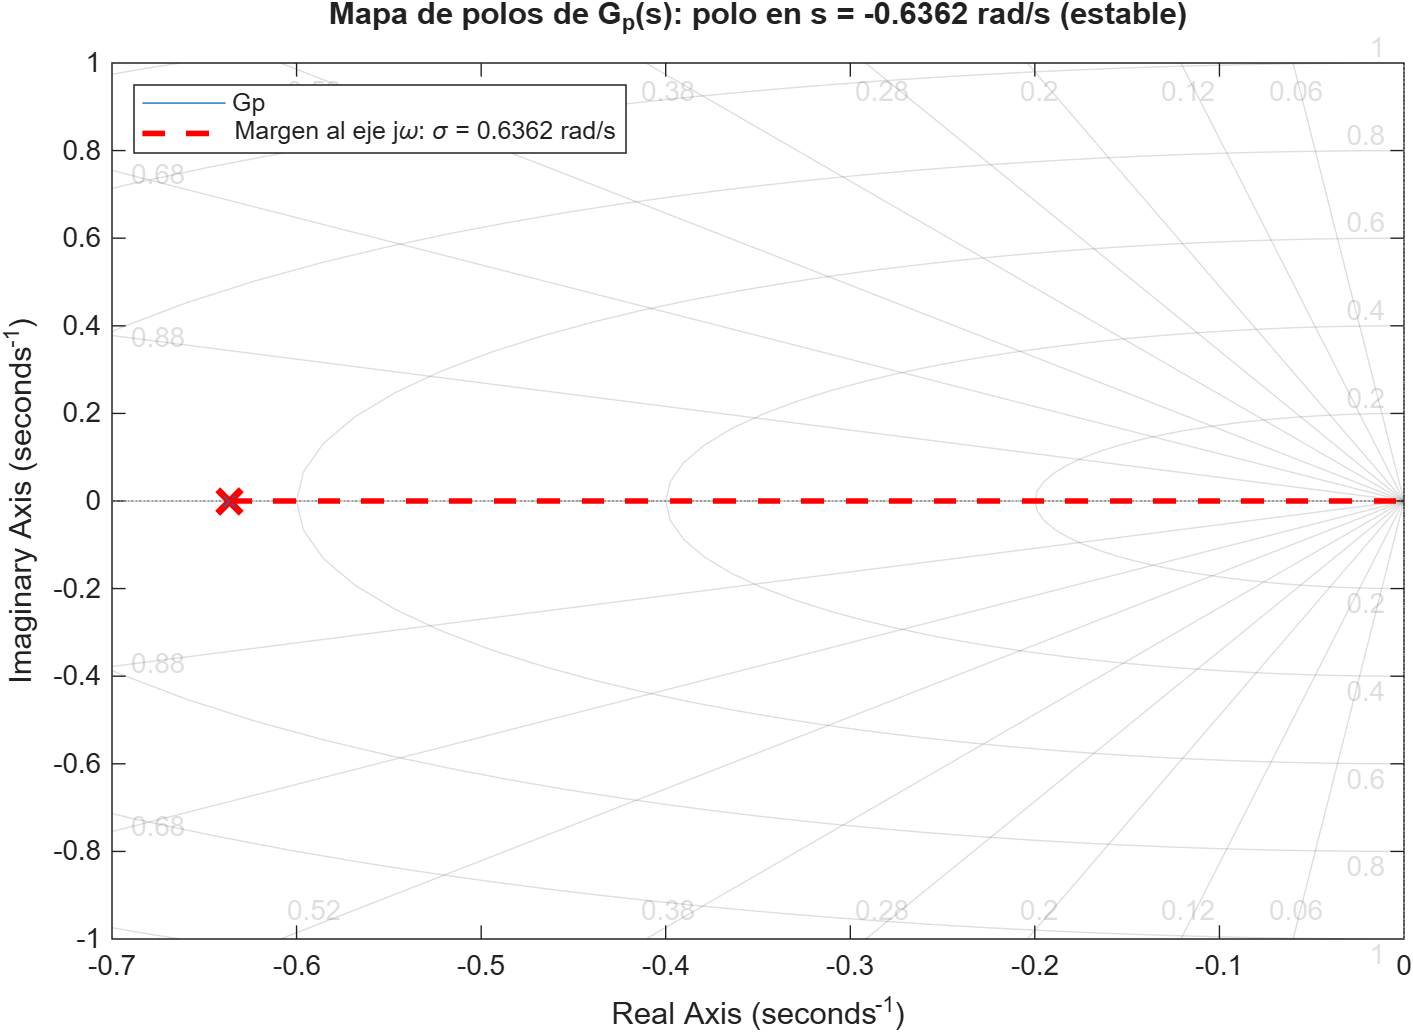
\includegraphics[width=0.9\columnwidth]{mapa_polos.png}
\caption{Mapa de polos de $G_p(s)$ con rejilla de amortiguamiento y frecuencia natural (\texttt{pzmap} + \texttt{sgrid}).}
\label{fig:polos}
\end{figure}

\subsection{Validación y análisis de residuos}
El modelo alcanza un ajuste de \SI{85.77}{\percent}, superior al criterio de la guía, con un RMSE de \SI{0.754}{cm}, del orden de la resolución práctica del HC-SR04. Contra la señal sin filtrar el ajuste baja solo a \SI{84.02}{\percent}, lo que indica que el filtro de mediana no ``fabrica'' el buen ajuste. Los resultados analíticos coinciden con la simulación por \texttt{lsim} con retardo de transporte (diferencia máxima \SI{0.03}{cm}). El mismo modelo implementado en Simulink (\texttt{Step} de \SI{50}{\micro\second} $\rightarrow$ \texttt{Transfer Fcn} $\rightarrow$ \texttt{Transport Delay} $\rightarrow$ suma de $y_0$) reproduce el ensayo con un ajuste de \SI{85.79}{\percent} y un RMSE de \SI{0.753}{cm} (Fig.~\ref{fig:simulink}).

\begin{figure}[t]
\centering
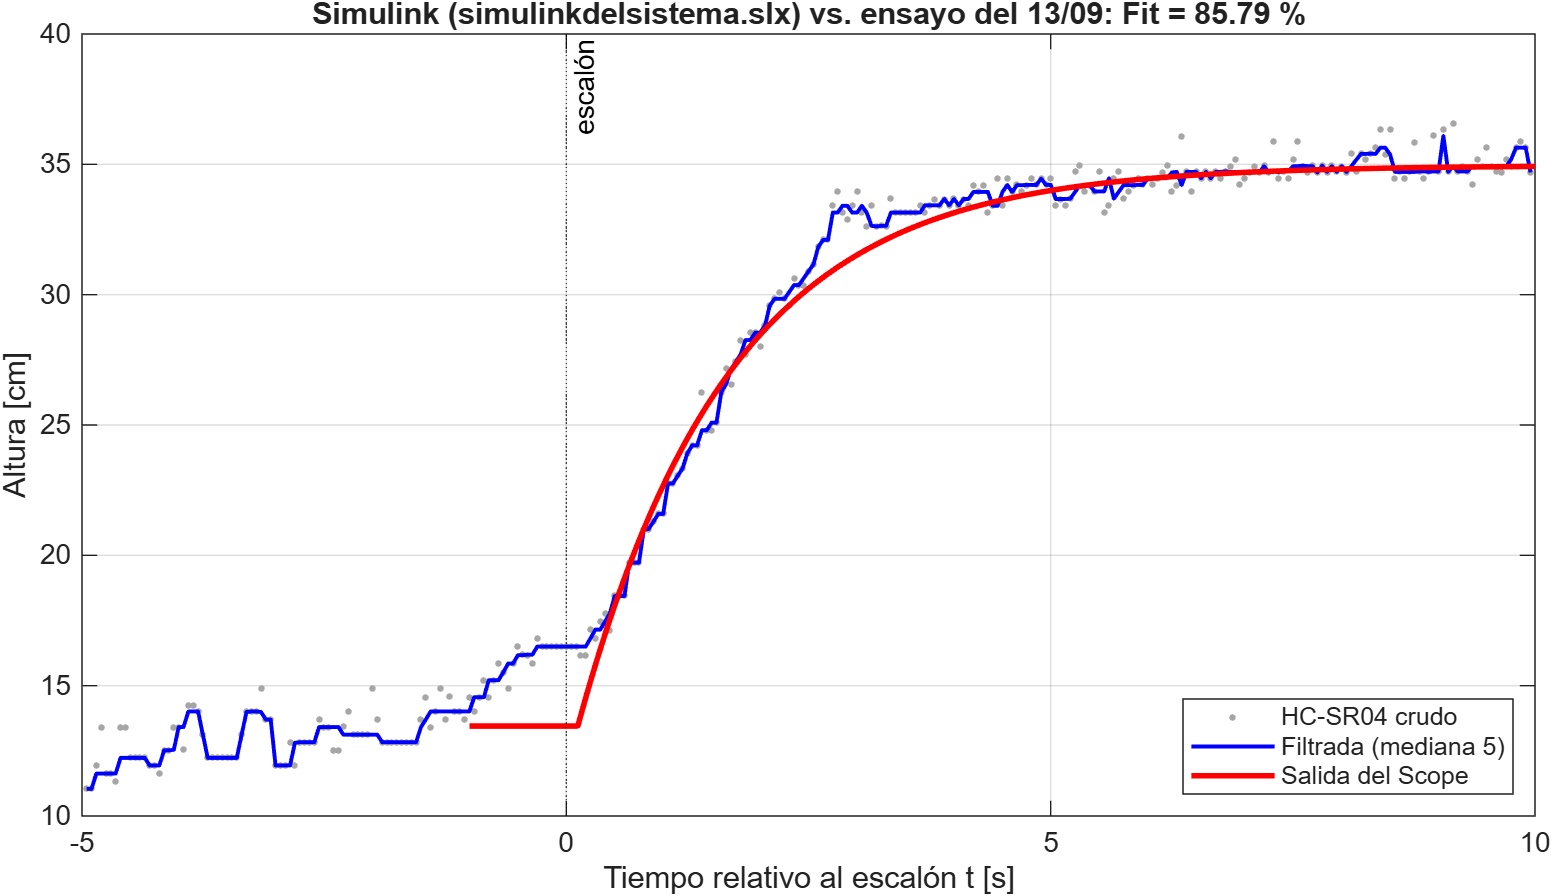
\includegraphics[width=\columnwidth]{simulink_vs_experimental.png}
\caption{Salida del Scope de \texttt{simulinkdelsistema.slx} superpuesta a la altura medida (figura generada con \texttt{ValidacionSimulink.m}).}
\label{fig:simulink}
\end{figure}

Los residuos (Fig.~\ref{fig:res}) se concentran en $\pm\SI{1}{cm}$ con media de \SI{0.27}{cm}, pero no son ruido blanco:
\begin{itemize}
\item En $t\approx 0$ el error llega a \SI{3.05}{cm}. Justo antes del escalón el carro ya había subido de \SI{13}{cm} a \SI{16.5}{cm} (Fig.~\ref{fig:fit3}): el punto de operación no estaba en reposo ($\dot y\neq 0$), mientras que el modelo parte del promedio $y_0$.
\item Entre \SI{1}{s} y \SI{1.6}{s} el modelo va ligeramente por encima de la medida, y entre \SI{2.5}{s} y \SI{3}{s} por debajo: la subida real tiene forma levemente sigmoidal, huella del segundo polo que el FOPDT desprecia.
\end{itemize}

\begin{figure}[t]
\centering
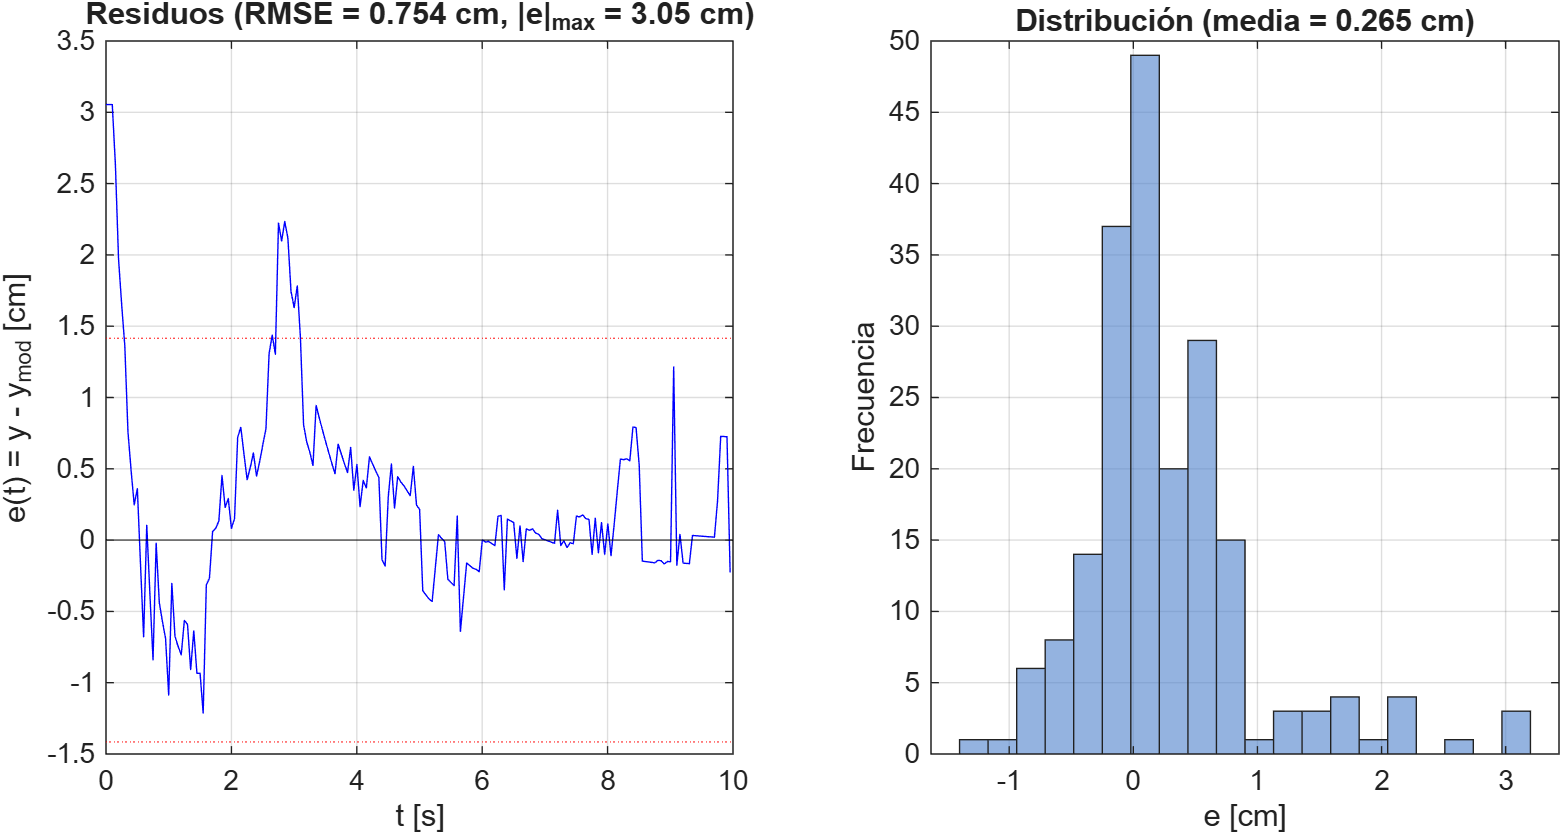
\includegraphics[width=\columnwidth]{fit3_residuos.png}
\caption{Residuos del modelo en el tiempo y su distribución.}
\label{fig:res}
\end{figure}

% ---------------------------------------------------------------------
\section{Discusión y análisis crítico}

\subsection{Limitaciones del modelo FOPDT}
El modelo es local: $K$ se midió entre \SI{13}{cm} y \SI{35}{cm} con un escalón de \SI{50}{\micro\second}. Por la relación cuadrática empuje--PWM, la ganancia cambia con el punto de operación; fuera de ese rango (cerca de la base o del travesaño) debe esperarse un error mayor. El FOPDT tampoco reproduce la zona muerta ni la saturación del recorrido.

\subsection{Fuentes de error}
\begin{itemize}
\item \textbf{Punto de operación.} La guía sugiere $y_0\approx\SI{20}{cm}$; el ensayo se hizo en $y_0=\SI{13.45}{cm}$, más cerca de la base, donde el efecto suelo es mayor, y con una deriva de $\approx\SI{3}{cm}$ antes del escalón. Se recomienda repetir el ensayo con $u_0$ ajustado para $y_0\approx\SI{20}{cm}$ y comprobar $\dot y\approx 0$ durante los \SI{5}{s} previos.
\item \textbf{Sensor ultrasónico.} El HC-SR04 tiene un haz de $\approx\SI{15}{\degree}$ y el carro es una tabla angosta: parte de los pulsos no rebota en el carro sino en el travesaño superior ($\approx$\SI{90}{cm}) o no regresa. Estas lecturas espurias explican los saltos aislados de la señal cruda y, en lazo cerrado, disparaban el \textit{failsafe} con el carro a \SI{30}{cm}. El firmware actualizado rechaza saltos físicamente imposibles (\SI{>12}{cm} en \SI{50}{ms}) salvo que tres lecturas consecutivas los confirmen, aplica una mediana de tres muestras y exige tres muestras consecutivas sobre \SI{85}{cm} para el \textit{failsafe}. Se recomienda además pegar una placa reflectora plana bajo el carro.
\item \textbf{Cuantización temporal.} Con $T_s=\SI{50}{ms}$, el tiempo muerto identificado (\SI{0.119}{s}) equivale a solo 2.4 muestras, por lo que su incertidumbre es del orden de $\pm T_s/2$.
\item \textbf{Variación de la alimentación.} El empuje depende de la tensión que recibe el ESC; una caída de la fuente durante el ensayo modifica $K$.
\end{itemize}

\subsection{Comparación con otros métodos}
Los métodos Fit~1 (tangente de Ziegler--Nichols) y Fit~2 (tangente más punto del \SI{63.2}{\percent}) dependen de trazar la tangente en el punto de inflexión, muy sensible al ruido del ultrasonido. Fit~3 usa solo dos cruces de nivel interpolados sobre la señal filtrada, lo que lo hace más robusto y reproducible con datos ruidosos~\cite{smith}. [COMPLETAR si se calculan Fit~1 y Fit~2: tabla comparativa de $K,\tau,t_0$ y Fit.]

\subsection{Implicaciones para el diseño del PID (Etapa 2)}
La razón $t_0/\tau=0.076$ es pequeña, de modo que la planta es fácil de controlar y admite una sintonía rápida. Con la regla SIMC~\cite{skogestad} y una constante de tiempo de lazo cerrado $\tau_c=\SI{0.8}{s}$:
\begin{equation}
K_p=\frac{\tau}{K(\tau_c+t_0)}=\SI{3.98}{\micro\second/cm},\quad
T_i=\min\{\tau,\,4(\tau_c+t_0)\}=\SI{1.57}{s},
\end{equation}
es decir, $K_p\approx 4.0$ y $K_i=K_p/T_i\approx\SI{2.5}{\micro\second/(cm\,s)}$, con una pequeña acción derivativa sobre la medida ($K_d=\SI{0.3}{\micro\second\,s/cm}$) y anti-\textit{windup}. En simulación sobre el modelo identificado, incluyendo el ruido y los ecos espurios del sensor, esta sintonía produce un sobreimpulso cercano al \SI{2}{\percent} y un tiempo de establecimiento de $\approx\SI{2}{s}$. La validación experimental en el banco queda para la Etapa~2.

% ---------------------------------------------------------------------
\section{Conclusiones}
\begin{itemize}
\item Se identificó el modelo $G_p(s)=0.4302\,e^{-0.1188s}/(1.5719s+1)$ del monóptero alrededor de $(u_0,y_0)=(\SI{1762}{\micro\second},\SI{13.45}{cm})$, con un ajuste de \SI{85.77}{\percent} y un RMSE de \SI{0.754}{cm}, cumpliendo el criterio de aceptación (Fit $\geq\SI{80}{\percent}$).
\item La planta es estable en lazo abierto (polo en \SI{-0.636}{rad/s}) y está dominada por un polo; el tiempo muerto es pequeño frente a la constante de tiempo.
\item El análisis de residuos revela una deriva del punto de operación antes del escalón y una dinámica de segundo orden no modelada; ambos efectos limitan el ajuste y se corrigen repitiendo el ensayo en un hovering estable cerca de \SI{20}{cm}.
\item Las lecturas espurias del HC-SR04 son la principal fuente de error de medición y deben filtrarse en el firmware antes de cerrar el lazo.
\item El modelo cuantitativo obtenido permite sintonizar analíticamente el PID de la Etapa~2.
\end{itemize}

\begin{thebibliography}{9}
\bibitem{smith} C. A. Smith y A. B. Corripio, \textit{Principles and Practice of Automatic Process Control}, 3.\textsuperscript{a} ed. Hoboken, NJ, EE.~UU.: Wiley, 2006.
\bibitem{ogata} K. Ogata, \textit{Ingeniería de Control Moderna}, 5.\textsuperscript{a} ed. Madrid, España: Pearson, 2010.
\bibitem{skogestad} S. Skogestad, ``Simple analytic rules for model reduction and PID controller tuning,'' \textit{J. Process Control}, vol.~13, no.~4, pp.~291--309, 2003.
\bibitem{guia} J. D. Guillot Fula, ``Guía de laboratorio — Proyecto Etapa 1: caracterización experimental y modelado dinámico del monóptero,'' Universidad del Magdalena, 2026.
\end{thebibliography}

% ---------------------------------------------------------------------
\appendices
\section{Archivos del proyecto}
\begin{itemize}
\item Datos: \texttt{02\_datos/datos\_escalon\_20260913\_193329.csv}.
\item Código MATLAB: \texttt{03\_matlab/IdentificacionFIT3.m}, \texttt{Polosmonocopter.m}, \texttt{simulinkdelsistema.slx}.
\item Firmware del ensayo: \texttt{04\_firmware/ensayo\_escalon\_original}; firmware actualizado: \texttt{04\_firmware/arduino\_uno} y \texttt{04\_firmware/esp32}.
\item [COMPLETAR] Fotografías del montaje durante el ensayo.
\end{itemize}

\end{document}
